\documentclass[a4paper, 14pt]{extarticle}
\setlength{\parindent}{0.75cm}
\usepackage[utf8]{inputenc}
\usepackage[T2A]{fontenc}
\usepackage[warn]{mathtext}
\usepackage{amssymb}
\usepackage{amsmath}
\usepackage[russian]{babel}
\usepackage{scrextend}
\usepackage{multirow}
\usepackage{hhline}
\usepackage{float}
\usepackage{multicol}
\usepackage{graphicx}
\usepackage{placeins}
\usepackage{makecell}
\usepackage{setspace}
\usepackage{ragged2e}
\usepackage{titlesec}
\usepackage{listings}
\usepackage{svg}
\usepackage{xcolor}
\usepackage{tocloft}
\usepackage[left=2cm,right=2cm, top=2cm,bottom=2cm,bindingoffset=0cm]{geometry}

\lstset{
  language=matlab,
  basicstyle=\ttfamily\small, % Шрифт и размер
  keywordstyle=\color{blue}, % Цвет ключевых слов
  stringstyle=\color{red}, % Цвет строк
  commentstyle=\color{green}, % Цвет комментариев
  identifierstyle=\color{black}, % Цвет идентификаторов (переменных, функций)
  showstringspaces=false,
  showspaces=false,
  showtabs=false,
  numbers=left, % Номера строк слева
  numbersep=5pt, % Расстояние от текста до номеров строк
  breaklines=true, % Перенос длинных строк
  breakatwhitespace=true, % Перенос только по пробелам
  frame=single, % Добавить рамку вокруг кода
  rulecolor=\color{gray}, % Цвет рамки
  backgroundcolor=\color{gray!5}, % Цвет фона (легкий серый)
  captionpos=b, % Положение подписи (bottom)
  tabsize=2 % Размер табуляции
}

\newcommand{\myappendixsection}[1]{%
  \section*{\large #1}
}

			
\usepackage[T2A]{fontenc}			
\usepackage[russian]{babel}			
\usepackage[utf8x]{inputenc}			
\usepackage[scaled=0.95]{PTSans}			
\usepackage{graphicx}			
%\usepackage[usenames,dvipsnames]{xcolor}			
\usepackage{algorithm}			
\usepackage{algorithmic}			
\usepackage{latexsym,amssymb,amsthm}			
%предметный указатель

\usepackage{multicol}

\newenvironment{theindex}{}{}

\usepackage[xindy]{imakeidx}

\renewenvironment{theindex}{%
	
	
	
	\vspace*{-25pt}\begin{center}\color{blue}\Large Предметный указатель\end{center}%
	
	
	
	\def\item{\par\hangindent 0pt\parindent0pt}%
	
	\def\subitem{\par\hangindent10pt\parindent10pt}%
	
	\def\subsubitem{\par\hangindent20pt\parindent20pt}%
	
	\def\indexspace{}%
	
	\begin{multicols}{2}
		
	}{\end{multicols} }



\makeindex[options=-L russian -C utf8]

\AtBeginDocument{%
	
	\let\originalindex\index
	
	\renewcommand{\index}[1]{\originalindex{\detokenize{#1}}}%
	
}

%конец предметного указателя			
\usepackage{ragged2e}			
\justifying			
\renewcommand{\raggedright}{\leftskip=0pt \rightskip=0pt plus 0cm}			
\hyphenpenalty=5 			
\exhyphenpenalty=10000			
\doublehyphendemerits=2			
\finalhyphendemerits=500			
\uchyph=0			
\renewcommand{\algorithmicrequire}{\textbf{Вход:}}			
\renewcommand{\algorithmicensure}{\textbf{Выход:}}			
\renewcommand{\algorithmiccomment}{{\color{gray} //}}			
%Здесь располагаются все макросы для всякой математики и алгоритмов -			
%\let\em\it			
\def\em#1{{\it\color{blue}#1}}
\def\NB#1{{\bf\color{brown}#1}}
\def\RS{{\color{red}\bf*}}	
\def\BS{{\color{blue}\bf*}}		
%\def\eqed{\tag{\qed}}			
\def\Boxed#1{#1}			
\def\odmkey#1#2{{\it\color{red} #1}\index{#2}}			
\let\emptyset\varnothing			
\def\Set#1#2{\left\{ #1 \mid #2 \right\}}			
\let\Equiv\Longleftrightarrow			
\def\Assign{\operatorname{:=}}			
\def\Pointer{\operatorname{\uparrow\!}}			
\def\Is{\operatorname{\colon}}
\def\plusplus{\operatorname{+\!+}}			
\def\Def{\stackrel{\text{Def}}{=}}			
\def\SubsetNE{\varsubsetneq}%\stackrel{\ne}{\subset}}			
\def\SubsetOne{\stackrel{+1}{\subset}}			
\def\dDef{\operatorname{::=}}			
\def\A#1#2{\forall\,#1\ \left(#2\right)}			
%\def\A#1#2{\forall\,#1\ \linebreak[2]\left(#2\right)}			
\def\dA#1#2{\forall\,#1\cdots #2}			
\def\Alg#1#2{\left\langle #1;#2\right\rangle}			
\def\Bl#1{\mathbf{#1}}			
\def\hy#1{\left( #1 \right)}			
\def\DIVC#1#2{\left\langle #1 , #2\right\rangle}
\def\divC#1#2{\left\langle #1 , #2\right\rangle}			
\def\DIVI#1#2{#1\in #2}			
\def\E#1#2{\exists\,#1\ \left(#2\right)}			
%\def\E#1#2{\exists\,#1\ \linebreak[2]\left(#2\right)}			
\def\To#1{\stackrel{#1}{\longrightarrow}}			
\def\ToC#1{\stackrel{#1}{,}}			
\def\ToS#1{\stackrel{#1}{\sim}}			
\def\ToE#1{\stackrel{#1}{=}}			
\def\Tuple#1#2#3{{#1}_{#2},\dots,{#1}_{#3}}			
\def\dTuple#1#2#3{{#1}_{#2}\dots{#1}_{#3}}			
\let\Impl\Longrightarrow			
\let\Impll\Longleftarrow			
\def\And{\operatorname{\,\&\,}}			
\def\Or{\,\vee\,}			
\def\Wedge{\,\wedge\,}			
\def\BigOr{\bigvee}			
\def\BigAnd{\bigwedge}			
\def\nat{\operatorname{\rm nat}}			
\def\sgn{\operatorname{\rm sgn}}			
\def\func{\operatorname{\rm func}}			
\def\ker{\operatorname{\rm ker}}			
\def\Im{\operatorname{\rm Im}}			
\def\Dom{\operatorname{\rm Dom}}			
\def\Ob{\operatorname{\rm Ob}}			
\def\Mor{\operatorname{\rm Mor}}			
\def\SetCat{\operatorname{\rm Set}}			
\def\OrSet{\operatorname{\rm OrSet}}			
\def\Aut{\operatorname{\rm Aut}}			
\def\End{\operatorname{\rm End}}			
\def\Gr{\operatorname{\rm Gr}}			
\def\Suc{\operatorname{\rm Suc}}			
\def\card{\operatorname{\rm card}}			
\def\pr{\operatorname{\rm pr}}			
\def\MOD{\operatorname{\rm\bf mod}}			
\def\DIV{\operatorname{\rm\bf div}}			
\def\Lrf#1{\lfloor #1 \rfloor}			
\def\lrle#1{\langle #1 \rangle}			
\def\llrle#1{\langle {\text{#1}} \rangle}			
\def\Map#1#2#3{{#1}\colon{#2}\nolinebreak\to\nolinebreak{#3}}			
\def\MapI#1#2#3{{#1}\colon{#2}\in{#3}}			
\def\Rule#1#2#3{\frac{#1}{#2}\,#3}			
\def\Seq#1#2#3{#1 \vdash_{#3} #2}			
\def\Prog#1#2#3{\{#1\}\,#2\,\{#3\}}			
\def\Not{\neg}			
\def\demo{\noindent $\triangleright$ \vskip 3 em \par\hfill$\triangleleft$}			
\DeclareMathOperator{\Eq}{Eq}			
\DeclareMathOperator{\Unify}{Unify}			
\DeclareMathOperator{\Antilex}{Antilex}			
\DeclareMathOperator{\Reverse}{Reverse}			
\DeclareMathOperator{\Fano}{Fano}			
\DeclareMathOperator{\Med}{Med}			
\DeclareMathOperator{\Huffman}{Huffman}			
\DeclareMathOperator{\Up}{Up}			
\DeclareMathOperator{\Down}{Down}			
\DeclareMathOperator{\KCC}{KCC}			
\DeclareMathOperator{\NewNode}{NewNode}			
\DeclareMathOperator{\Find}{Find}			
\DeclareMathOperator{\New}{new}			
\DeclareMathOperator{\Dispose}{dispose}			
\DeclareMathOperator{\Delete}{Delete}			
\DeclareMathOperator{\BT}{BT}			
\DeclareMathOperator{\Last}{last}			
\DeclareMathOperator{\Selectmax}{Selectmax}			
\DeclareMathOperator{\Sort}{Sort}			
\DeclareMathOperator{\FD}{FD}			
\DeclareMathOperator{\Length}{Length}			
\DeclareMathOperator{\Append}{Append}			
\DeclareMathOperator{\Eval}{Eval}			
\DeclareMathOperator{\TraverseTree}{TraverseTree}			
%Списки, etc			
\def\labelenumi{\theenumi}			
\def\theenumi{\arabic{enumi}.}			
\def\labelenumii{\theenumii}			
\def\theenumii{\arabic{enumii})}			
\def\p@enumii{\theenumi}			
\def\labelenumiii{\theenumiii.}			
\def\theenumiii{\roman{enumiii}}			
\def\p@enumiii{\theenumi(\theenumii)}			
\def\labelenumiv{\theenumiv.}			
\def\theenumiv{\Alph{enumiv}}			
\def\p@enumiv{\p@enumiii\theenumiii}			
%нумерация			
%\numberwithin{equation}{chapter}			
%\numberwithin{algorithm}{chapter}			
%\numberwithin{figure}{chapter}			
%\renewcommand\thesection       {\thechapter.\arabic{section}}			
%\floatname{algorithm}{Алгоритм}			
%\renewcommand{\algorithmicrequire}{\textbf{Вход:}}			
%\renewcommand{\algorithmicensure}{\textbf{Выход:}}			
\let\cal\mathcal			
\let\Bbb\mathbb			
\let\leq\leqslant			
\let\le\leqslant			
\let\geq\geqslant			
\let\ge\geqslant			
\def\rmb#1{#1 \linebreak #1}			
\def\rmbb#1{#1 \\ #1}			
%% М. Лебедев, конец августа 2010			
\def\sign{\operatorname{\rm sign}}			
%% from class odm2007			
%\newtheorem*{theorem}{ТЕОРЕМА}			
%\newtheorem{vartheorem}{ТЕОРЕМА}			
%\newtheorem*{corollary}{\begin{corollary}}			
%\newtheorem{varcorollary}{\begin{corollary}}			
%\newtheorem*{lemma}{ЛЕММА}			
%\newtheorem{varlemma}{ЛЕММА}			
%\newtheorem*{ground}{Обоснование}			
%\def\endground{\qed\endtrivlist\@endpefalse }			
%\newtheorem*{example}{Пример}			
%\def\endexample{\qed\endtrivlist\@endpefalse }			
\def\clip#1{\bgroup\par\addvspace{7pt plus 3pt minus 3pt}%			
	\leavevmode\lower 3pt\hbox{\sffamily\bfseries #1} \hrulefill\par\nopagebreak\small} %\hrulefill\par\nopagebreak}			
\def\endclip{\par\nopagebreak\addvspace{3pt}\hrule width130mm\egroup%			
	\addvspace{12pt plus 3pt minus 3pt}}			
\def\remark{\par{\bf \color{brown} Замечание.}}			
\def\endremark{\par}			
\def\digress{\begin{small}
\par{\bf \color{brown} Отступление.}}			
	\def\enddigress{\end{small}\par}			
%\def\example{\par\addvspace{9pt plus 1pt minus 3pt}{\sffamily\bfseries Пример}\par\nopagebreak}			
%\def\endexample{\par\addvspace{9pt plus 1pt minus 3pt}}			
\def\example{\par{\bf \color{brown} Пример.}}			 
\def\endexample{\par}			
\def\examples{\par{\bf \color{brown} Примеры.}}			
\def\endexamples{\par}			
\def\prototheorem#1{\par{\bf #1}\bgroup\it}			
\def\endprototheorem{\par\egroup}			
\def\theorem{\prototheorem{\color{brown} Теорема.}}			
\def\endtheorem{\endprototheorem}			
\def\corollary{\prototheorem{\color{brown} Следствие.}}			
\def\endcorollary{\endprototheorem}			
\def\lemma{\prototheorem{\color{brown} Лемма.}}			
\def\endlemma{\endprototheorem}			
%\def\proof{\par\addvspace{12pt plus 3pt minus 3pt}{\sffamily\bfseries\small %Д{\scriptsize\uppercase{оказательство}}}\par\nopagebreak}			
%\def\proof{\par\addvspace{12pt plus 3pt minus 3pt}{\sffamily\bfseries\small %Д{\scriptsize\uppercase{оказательство}}}\quad\nopagebreak}			
\def\proof{\par{\bf\color{brown} Доказательство.}}			
\def\endproof{\hfill\qed\par}			
%\def\proofsection#1{\par{\small $\mathsf{\left[\:\text{{\sf#1}}\:\right]}$}\;}			
\def\proofsection#1{\par{\color{brown}\sffamily\small  [\;}{\sffamily\small\color{brown} #1}{\sffamily\small\color{brown}\;]}\;}			
\def\eqed{%			
	\gdef\tagform@##1{\maketag@@@{\ignorespaces##1\unskip}}%			
	\tag{\color{brown}\qed}%			
}			
\def\ground{\par{\bf\color{brown} Обоснование.}}			
\def\endground{\hfill\color{brown}\qed\par}			
% algorithms
%\newcounter{algorithm}[chapter]
\def\ext@algorithm{loa}
\def\fnum@algorithm{\algorithmname\ \thealgorithm}
\def\algorithmname{Алгоритм}
\def\thealgorithm{\thechapter.\arabic{algorithm}.}


\def\algorithm{%
	\def\@captionfont{\normalfont\sffamily\small}%
	\captionindent=-10\fill%
	\def\caption{\refstepcounter{algorithm}\@dblarg{\@caption{algorithm}}}%
	\def\@makecaption##1##2{\addvspace{12pt plus 3pt minus 2pt}\normalfont\sffamily\small{\bfseries ##1.} ##2}
	\small
}
\def\endalgorithm{\relax}


% citations
\def\@cite#1#2{{%
		\m@th\upshape\mdseries[{#1}{\if@tempswa, #2\fi}]}}
		
% 	% Стиль презентации			
% 	\usetheme{default}			
% 	\setbeamertemplate{navigation symbols}{}			
% 	\setbeamertemplate{footline}[page number]			
% 	\setbeamersize{text margin left = 6pt}			
% 	\setbeamersize{text margin right = 6pt}			
			
% %	\usepackage{epstopdf}			
% 	%\renewcommand{\algorithmiccomment}{ //}			
% 	\def\Reduce{\stackrel{*}{\leadsto}}			
% 	\DeclareMathOperator{\Clear}{Clear}			
% 	\DeclareMathOperator{\Conf}{Conf}			
% 	\DeclareMathOperator{\lcm}{lcm}			
% 	\def\Mod#1#2#3{#1\equiv #2 \,\left(\bmod\,#3\right)}			
% 	%\newtheorem{theorem}{ТЕОРЕМА}			
% %	\def\digress{\par{\bf Отступление.}}			
% %	\def\enddigress{\par}			
			
% 	\renewcommand{\algorithmiccomment}{ //}			
% 	\DeclareMathOperator{\GI}{Grey2Int}			
			
% 	\setbeamertemplate{frametitle continuation}{}			
% 	\def\TT{\text{T}}			
% 	\def\FF{\text{F}}			
% 	\DeclareMathOperator{\firstNeqSubTerms}{firstNeqSubTerms}			
				
% 	\DeclareMathOperator{\Partition}{Partition}			
% 	\DeclareMathOperator{\Quicksort}{Quicksort}			
			
% 	\DeclareMathOperator{\ChangeArray}{ChangeArray}			
% 	%\newtheorem{corollary}{\begin{corollary}}			
			
% 	\def\divI#1#2{#1 \in #2}			
% 	\DeclareMathOperator{\Ordering}{Ordering}			
% 	\setbeamertemplate{frametitle}			
% 	{\color{blue}\large\insertframetitle\par\vskip-6pt}			
	%%вставка для оглавления со страницами			
	%\makeatletter			
	%\long\def\beamer@section[#1]#2{%			
	%	\beamer@savemode%		
	%	\mode<all>%		
	%	\ifbeamer@inlecture		
	%	\refstepcounter{section}%		
	%	\beamer@ifempty{#2}%		
	%	{\long\def\secname{#1}\long\def\lastsection{#1}}%		
	%	{\global\advance\beamer@tocsectionnumber by 1\relax%		
	%		\long\def\secname{#2}%	
	%		\long\def\lastsection{#1}%	
	%		\addtocontents{toc}{\protect\beamer@sectionintoc{\the\c@section}{#2\hfill\the\c@page}{\the\c@page}{\the\c@part}%	
	%			{\the\beamer@tocsectionnumber}}}%
	%	{\let\\=\relax\xdef\sectionlink{{Navigation\the\c@page}{\noexpand\secname}}}%		
	%	\beamer@tempcount=\c@page\advance\beamer@tempcount by -1%		
	%	\beamer@ifempty{#1}{}{%		
	%		\addtocontents{nav}{\protect\headcommand{\protect\sectionentry{\the\c@section}{#1}{\the\c@page}{\secname}{\the\c@part}}}%	
	%		\addtocontents{nav}{\protect\headcommand{\protect\beamer@sectionpages{\the\beamer@sectionstartpage}{\the\beamer@tempcount}}}%	
	%		\addtocontents{nav}{\protect\headcommand{\protect\beamer@subsectionpages{\the\beamer@subsectionstartpage}{\the\beamer@tempcount}}}%	
	%	}%		
	%	\beamer@sectionstartpage=\c@page%		
	%	\beamer@subsectionstartpage=\c@page%		
	%	\def\insertsection{\expandafter\hyperlink\sectionlink}%		
	%	\def\insertsubsection{}%		
	%	\def\insertsubsubsection{}%		
	%	\def\insertsectionhead{\hyperlink{Navigation\the\c@page}{#1}}%		
	%	\def\insertsubsectionhead{}%		
	%	\def\insertsubsubsectionhead{}%		
	%	\def\lastsubsection{}%		
	%	\Hy@writebookmark{\the\c@section}{\secname}{Outline\the\c@part.\the\c@section}{2}{toc}%		
	%	\hyper@anchorstart{Outline\the\c@part.\the\c@section}\hyper@anchorend%		
	%	\beamer@ifempty{#2}{\beamer@atbeginsections}{\beamer@atbeginsection}%		
	%	\fi%		
	%	\beamer@resumemode}%		
	%			
	%\def\beamer@subsection[#1]#2{%			
	%	\ifbeamer@inlecture%		
	%	\refstepcounter{subsection}%		
	%	\beamer@ifempty{#2}{\long\def\subsecname{#1}\long\def\lastsubsection{#1}}		
	%	{%		
	%		\long\def\subsecname{#2}%	
	%		\long\def\lastsubsection{#1}%	
	%		\addtocontents{toc}{\protect\beamer@subsectionintoc{\the\c@section}{\the\c@subsection}{#2\hfill\the\c@page}{\the\c@page}{\the\c@part}{\the\beamer@tocsectionnumber}}%	
	%	\addtocontents{nav}{%		
	%		\protect\headcommand{\protect\beamer@subsectionentry{\the\c@part}{\the\c@section}{\the\c@subsection}{\the\c@page}{\lastsubsection}}%	
	%		\protect\headcommand{\protect\beamer@subsectionpages{\the\beamer@subsectionstartpage}{\the\beamer@tempcount}}%	
	%	\edef\subsectionlink{{Navigation\the\c@page}{\noexpand\subsecname}}%		
	%	\def\insertsubsection{\expandafter\hyperlink\subsectionlink}%		
	%	\def\insertsubsectionhead{\hyperlink{Navigation\the\c@page}{#1}}%		
	%	\Hy@writebookmark{\the\c@subsection}{#2}{Outline\the\c@part.\the\c@section.\the\c@subsection.\the\c@page}{3}{toc}%		
	%	\hyper@anchorstart{Outline\the\c@part.\the\c@section.\the\c@subsection.\the\c@page}\hyper@anchorend%		
	%	\beamer@ifempty{#2}{\beamer@atbeginsubsections}{\beamer@atbeginsubsection}%		
	%	\beamer@resumemode}		
	%\makeatother			
	%%конец вставки для оглавления			
			
	\def\Path#1#2{\langle {\stackrel{\rightarrow}{#1 , #2}}\rangle}			
	\DeclareMathOperator{\Init}{Init}			
	\DeclareMathOperator{\Relax}{Relax}			
	\DeclareMathOperator{\ExtractMin}{ExtractMin}			
	\DeclareMathOperator{\Aug}{Aug}			
%	{\color{blue}\large\insertframetitle\par\vskip-8pt}			
			
	\renewcommand{\algorithmicelsif}			
	{\algorithmicelse\algorithmicif}			
	\DeclareMathOperator{\Build}{Build}			
	\DeclareMathOperator{\Modify}{Modify}			
	\DeclareMathOperator{\Heapify}{Heapify}			
	\DeclareMathOperator{\MakeHeap}{MakeHeap}			
	\DeclareMathOperator{\IncElt}{IncElt}			
		
		
\def\DMref#1#2{\raisebox{0pt}{\color{blue}\underline{\hyperlink{#2}{#1}}}}		
			
\def\TODO#1{{\color{gray} TODO {#1}}}
\justifying
\renewcommand{\thesubsection}{\arabic{subsection}}

\begin{document}

\tableofcontents

\newpage

\section*{Введение}
\addcontentsline{toc}{section}{Введение}

Экологическое моделирование является неотъемлемым элементом современной экологии. Его методы применяются в рамках многих отраслей человеческой деятельности, например, в лесном и сельском хозяйстве. Одной из ключевых задач в этой области является моделирование численности популяций биологических видов. Получаемые результаты, в сочетании с данными наблюдений, имеют прикладное значение: в частности, они могут быть использованы для корректировки мер по сохранению исчезающих и уязвимых видов. Близким экологическому является демографическое моделирование, где нередко используются модели, адаптированные в соответствии со свойствами человеческих популяций для исследования социально-экономических процессов. Изучению ключевых моделей в этих двух смежных областях была посвящена значительная часть научно-исследовательской работы.

\newpage

\section*{Основная часть}
\addcontentsline{toc}{section}{Основная часть}

\subsection{Экспоненциальный рост}
Сперва были рассмотрены модели с ограничениями ресурсов и объёма популяции. Основой многих моделей динамики численности популяции является уравнение баланса для одного вида. Пусть функция $N(t)$ - численность вида в момент t, тогда тогда скорость изменения численности: 

\begin{center}
$\frac{dN}{dt}= births-deaths+migration.$
\end{center}

В простейшем случае пренебрегают миграцией; рождаемость и смертность представляются пропорциональными $N$ (они напрямую зависимы от численности), и для $ N(t)$ возникает решение вида:

\begin{center}
$\frac{dN}{dt}= bN-dN \implies N(t) = N_0e^{(b-d)t},$
\end{center}

где $b, d$ - положительные коэффициенты рождаемости и смертности, и начальная численность $N(0) = N_0$. Если $b>d$, то численность неограниченно растёт, а при $b<d$ убывает. Это - модель экспоненциального роста, предложенная английским учёным Томасом Мальтусом в 1798 году.

Строго говоря, ни одна популяция животных в природе не удовлетворяет мальтузианской модели в чистом виде, ведь существуют факторы, регулирующие рост численности: ограничения среды и ресурсов, а также взаимодействие с другими видами.

\subsection{Модели логистического роста}

\subsubsection{Простейшая модель}

Чтобы учесть эти факторы, бельгийский математик Пьер Франсуа Ферхюльст в 1838 году предложил модель логистического роста, которая была заново открыта и популяризирована американскими учеными Раймондом Пирлом и Лоуэллом Ридом в 1920-х годах. Исходное предположение для вывода уравнения при рассмотрении популяционной динамики звучит так: скорость размножения популяции пропорциональна её текущей численности и количеству доступных ресурсов.

\begin{center}
$\frac{dN}{dT} = rN(1-\frac{N}{K}),$
\end{center}

где $r$ (коэффициент рождаемости), $K$ (ёмкость среды) - положительные константы. Последняя определяется как количество доступных ресурсов, необходимых для поддержания жизни. Число рождений здесь представлено членом $r(1-\frac{N}{K})$, зависящим от $N$. Чем $N$ ближе к $K$, тем меньше прирост в данный момент времени. 

Если $N_0 = N(0)$ (задана начальная численность), то решение следующее:

\begin{center}
$N(t) = \frac{N_0Ke^{rt}}{[K+N_0(e^{rt}-1)]} \to K$ при $t \to \infty$
\end{center}

Если $N_0 < K$, то $N(t)$ просто монотонно возрастает до $K$, в то время как при $N_0 > K$ она монотонно сокращается до $K$. В первом случае существует качественное различие в зависимости от того, $N_0 > K/2$ или $N_0 < K/2$; при $N_0 < K/2$ кривая имеет сигмоидную форму, что обычно и наблюдается.

\begin{figure}[H]
    \centering
    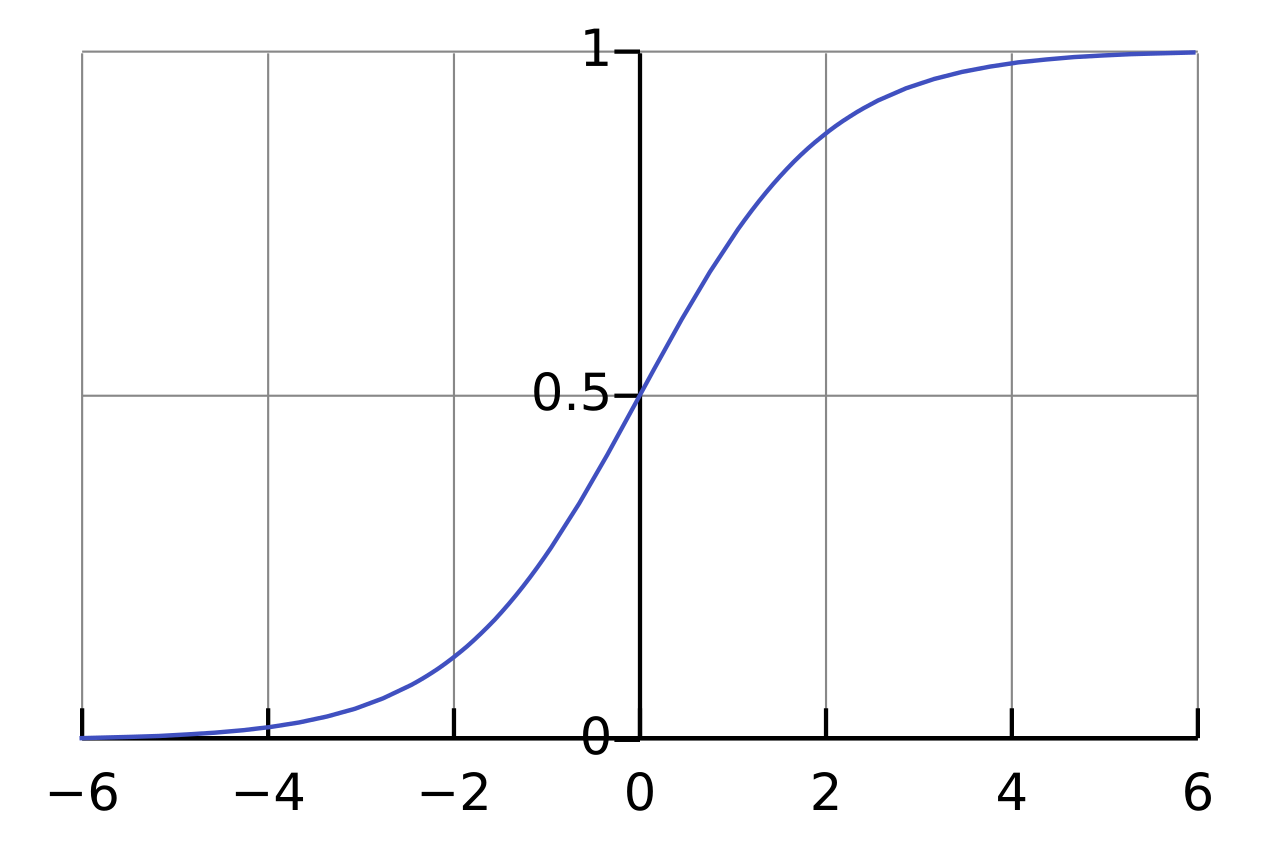
\includegraphics[width=1\linewidth]{log_curve.png} 
    \caption{Логистическая кривая для $K = 1, P_0 = 0,5, r = 1$}
\end{figure}

Логистическое уравнение - это основа для класса популяционных моделей с зависимым от плотности населения регуляторным механизмом – компенсацией в ответ на перенаселенность: при приближении численности населения к пределу рост теряет интенсивность, то есть насыщается.

Однако, более реалистичным ограничением численности популяции является изменяющееся во времени в зависимости от числа ресурсов. Следующая модель усложняет логистический рост, делая ёмкость среды переменной.

\subsubsection{Модель с производством ресурсов}

Для земледельческого общества характер потребления отличается от животных тем, что земледельцы потребляют производимые ими же ресурсы, то есть ёмкость среды $K$ не является постоянной величиной, а зависит от посевных площадей, которые, в свою очередь, зависят от численности населения.

Пусть $N(t)$ - численность популяции в момент времени $t$, а $K(t)$ - запасы зерна после сбора урожая, исчисляемые количеством минимальных годовых пайков. Площадь посевов, а следовательно, и урожай зависит от численности населения и при возрастании населения стремится к некоторой константе $a$, определяемой максимальной посевной площадью. Формула для урожая:

\begin{center}
$P = \frac{aN}{N+d},$
\end{center}

где $a$ и $d$ - некоторые константы. Для описания динамики населения используем логистическое уравнение:

\begin{center}
$\frac{dN}{dt} = rN\left(1 - \frac{N}{K}\right) \quad$
\end{center}

Поскольку за год расходуется $N$ пайков, то прирост запасов будет равен:

\begin{center}
$\frac{dK}{dt} = P - N = \frac{aN}{N+d} - N \quad$
\end{center}

Эта система дифференциальных уравнений имеет положение равновесия, когда население и запасы остаются постоянными. Из условия $\frac{dN}{dt} = 0$ и $\frac{dK}{dt} = 0$ получаем тривиальный случай $N = K = 0$, и также $\frac{aN}{N+d} - N = 0 \implies \frac{a}{N+d} = 1 \implies a = N + d$, и равновесие: $N_0 = K_0 = a - d$ (при $a>d$).

Если в формуле для производной $\frac{dP}{dN}$ устремить $N$ к 0, то получим, по правилу дифференцирования частного, $\frac{a}{d}$ - урожай (в количестве пайков), получаемый одним земледельцем в благоприятных условиях. Величина $q = \frac{a}{d}$ показывает, сколько человек (включая себя) может в хороших условиях прокормить один земледелец. 

Выразим $a$ и $d$ через $q$ и $N_0$: $d = \frac{N_0}{q-1}, \quad a = \frac{qN_0}{q-1}.$
 
В этой модели мы имеем две константы, имеющие реальный смысл: $r$ - максимальный естественный прирост населения ($0.01 < r < 0.02$), $q$ - продуктивность земледелия (предполагается в пределах $1.2 < q < 2$).

Данная пара уравнений уже способна описывать более сложное поведение, чем обычная логистическая модель, в частности — колебания численности.

В случае, когда начальное население мало, первый цикл может быть намного длиннее обычного. Численность населения с запозданием реагирует на уменьшение экологической ниши и продолжает расти в то время, когда экологическая ниша (совокупность имеющихся и производимых ресурсов) сокращается.

В результате происходит демографическая катастрофа; за короткое время население может уменьшиться в 2-4 раза. После катастрофы, в условиях изобилия свободных посевных площадей, население снова возрастает, но чрезмерный рост приводит к новой катастрофе. Каждый следующий цикл по протяженности приближается к некоторому стандартному периоду, и каждый раз падение численности населения имеет меньшие масштабы; колебания постепенно затухают.

\begin{figure}[H]
    \centering
    
\includegraphics[width=.85\linewidth]{log_agrar.png}  
    \caption{Результаты при $r = 0.015, a = 650, d = 500, N_0 = 100, K_0 = 50.$}
\end{figure}

\begin{figure}[H]
    \centering
    
\includegraphics[width=.85\linewidth]{dem_cat.png}  
    \caption{Продовольственная катастрофа и падение численности населения в момент $t \sim 20$ при $r = 0.02, a = 130, d = 100, N_0 = 50, K_0 = 1000.$}
\end{figure}

Реализация модели в MATLAB вынесена в Приложение 1. 

Модель с ёмкостью среды, зависящей от других параметров, несмотря на её преимущества, определенно не исчерпывающая. Уже в этой модели неявно возникает запоздание, ведь урожай зависит от населения в прошлом. Это главная идея следующей модели. Учёт задержки вступления живых существ в репродуктивный возраст, внедряемый в уравнения Ферхюльста, является значительным улучшением, которое стоит рассмотреть подробнее.

\subsubsection{Логистическая модель с запаздыванием}

Разумно полагать, что рождаемость, например, зависит не от текущего, а от прошлогоднего урожая. Предположим, что скорость роста популяции в момент времени $t$ зависит не от текущей численности $N(t)$, а от численности в некоторый момент в прошлом $t - \tau $, где $\tau$ — константа запаздывания.

Тогда логистическое уравнение принимает вид:

\begin{center}
$\dfrac{dN}{dt} = rN(t)\cdot[1 - \frac{N(t - \tau)}{K}]$
\end{center}

Автор этого уравнения - американский эколог Хатчинсон. Оно является простейшим способом учесть задержку; более сложные модели учитывают усреднение по времени и используют интегро-дифференциальные уравнения. 

Стационарные точки этой модели ($N = 0$ и $N = K$) совпадают с точками обычной логистической модели. Однако её поведение принципиально иное: при увеличении задержки $\tau$ устойчивое равновесие $N = K$ теряет устойчивость, и в системе возникают незатухающие колебания (предельные циклы).

Это хорошо согласуется с данными наблюдений, например, за фитопланктоном на хемостатах, бабочками-листовёртками, жуками-короедами. Однако, размеры популяций более сложных животных, например, зайцев или леммингов, практически всегда рассматривают как одновременно зависящие от количества хищников, и в то же время опосредующие их численность. Системы подобной структуры составляют класс моделей <<хищник-жертва>>.

В реальных экосистемах влияние перенаселения на рождаемость и смертность действительно ощущается с некоторой задержкой: например, истощение ресурсов сегодня скажется на способности выкормить потомство только через несколько лет. Именно для исследования численности популяций, учитывающего влияние подобных факторов, используются модели с задержкой.

\begin{figure}[H]
    \centering
    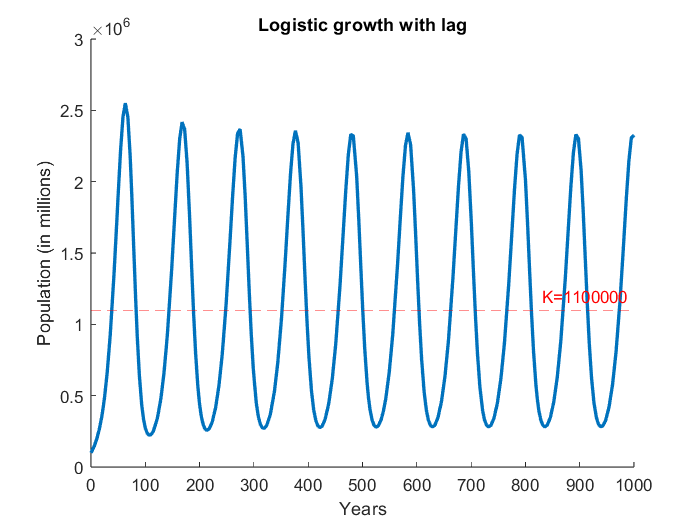
\includegraphics[width=1\linewidth]{log_lag.png}
    \caption{Модель с запаздыванием, параметры: $r = 0.07, K = 1100000, \tau = 25, N_0 = 100000, T = 1000$. Наблюдаются устойчивые колебания.}
\end{figure}

Анализ демографических процессов невозможен без учёта состава населения. Ключевым для исследований населения методами демографии, экологии и статистики является введение в модель возрастной структуры или создание отдельной модели для отдельного её рассмотрения, что удобнее, шире распространено и зачастую полезнее. Для упрощенного представления изменения структуры населения в демографии и для строгого описания жизненного цикла животных в экологии используют матричные модели популяций. Также существует способ на основе интегро-дифференциальных уравнений, который продемонстрирован далее.

\subsection{Введение возрастной структуры}

Все рассмотренные до сих пор модели, будь то модели Мальтуса, Ферхюльста или Хатчинсона, оперируют единым (агрегированным) параметром — общей численностью популяции \( N(t) \). Однако для детального демографического прогноза, особенно для человеческих популяций, принципиально важно учитывать её возрастную структуру. Очевидно, что рождаемость и смертность распределены по возрастам неравномерно: способность к воспроизводству сосредоточена в определенной возрастной группе, а смертность, как правило, высока среди самых молодых и самых старых членов популяции.

Для учёта этого фактора используется модель, описываемая не обыкновенным дифференциальным уравнением, а линейным уравнением в частных производных. Эта модель известна как уравнение фон Ферстера (или Маккендрика–фон Ферстера).

Пусть \( n(t, a) \) — плотность популяции в момент времени \( t \) в возрасте \( a \). Это означает, что число особей в возрасте от \( a \) до \( a + da \) в момент \( t \) равно \( n(t, a) \, da \). 

Пусть \( \mu(a) \geq 0 \) — возрастозависимая функция смертности, а \( b(a) \geq 0 \) — возрастозависимая функция рождаемости.

Тогда, например, число особей в возрасте а, которое умирает в течение небольшого отрезка времени dt, равно $\mu(a)n(t, a)dt$. То есть, умирает часть населения, соразмерная плотности населения в некотором возрасте и умноженная на значение функции смертности в момент t.

Динамика числа особей описывается следующим образом:

\begin{equation}
\frac{\partial n}{\partial t} + \frac{\partial n}{\partial a} = -\mu(a) n.
\label{eq:partials}
\end{equation}

Уравнение имеет наглядную интерпретацию: изменение численности данной возрастной когорты со временем (\( \partial n / \partial t \)) происходит из-за двух процессов — старения (\( \partial n / \partial a \)) и смерти (\( -\mu n \)).

Уравнение \eqref{eq:partials} требует задания начального условия (возрастная структура в начальный момент времени, то есть уже существующие особи):

\[
n(0, a) = n_0(a),
\]

и граничного условия (число новорождённых при возрасте $a = 0$), которое задаётся функцией рождаемости:

\begin{equation}
n(t, 0) = \int_{0}^{\infty} b(a) \, n(t, a) \, da.
\label{eq:boundary}
\end{equation}

Рассмотрим условие \eqref{eq:boundary}. Здесь $n(t, a) da$ — это число особей в момент времени $t$ в возрастном интервале от $a$ до $a + da$, $b(a)$ — рождаемость (число детей в год на женщину возраста a). То есть, $b(a)n(t, a) da$ — это общее число потомков, произведенных за единицу времени всей когортой возраста $[a, a+da]$. 

Проще говоря, это столбик на возрастной гистограмме, показывающий число людей в некоторой возрастной когорте, чья ширина $\Delta d \to 0$.

\begin{figure}[H]
    \centering
    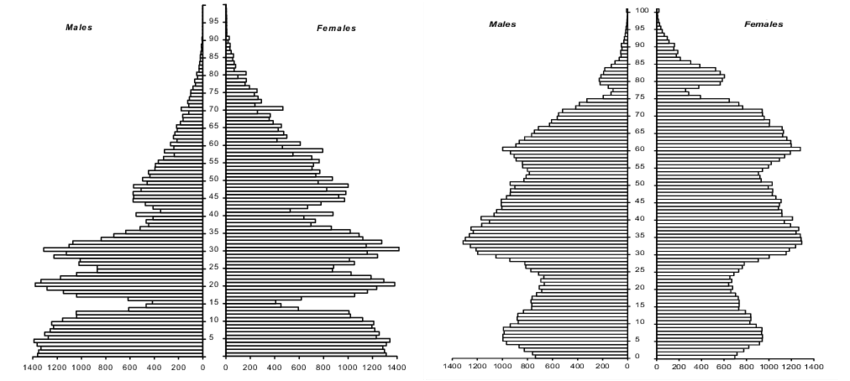
\includegraphics[width=1\linewidth]{rus_pop.png}
    \caption{Возрастная структура населения России в 1959 и в 2021.}
\end{figure}

Интеграл $\int_0^\infty b(a)n(t, a) da$ — сумма вклада когорт по всем репродуктивным возрастам. Иными словами, это общее число новорожденных в единицу времени в момент $t$. Именно это число и задается граничным условием как $n(t, 0)$ — плотность новорожденных в возрасте 0.

Решение уравнения \eqref{eq:partials} методом характеристик приводит к следующим выражениям:

Для когорт, существовавших в начальный момент (\( a > t \)):

\begin{equation}
n(t, a) = n_0(a - t) \, \exp\left( -\int_{a-t}^{a} \mu(s) \, ds \right)
\label{eq:sol_existing}
\end{equation}

Это решение описывает судьбу тех, кто уже жил при \( t = 0 \). Чтобы найти их число в момент \( t \), берётся начальное число в возрасте \( a - t \) и умножаем на вероятность дожить от возраста \( a-t \) до возраста \( a \).

Для когорт, родившихся после начального момента (\( a < t \)):

\begin{equation}
n(t, a) = n(t - a, 0) \, \exp\left( -\int_{0}^{a} \mu(s) \, ds \right)
\label{eq:sol_newborn}
\end{equation}

А это решение описывает родившихся после \( t = 0 \). Их число в момент \( t \) равно числу родившихся в момент \( t - a \), умноженному на вероятность дожить от рождения до возраста \( a \). 

Полезно ввести следующее обозначение: пусть $B(a) = b(a) \cdot \exp\left(-\int_0^a \mu(s)\, ds\right)$ — функция воспроизводства, показывающая среднее число потомков, произведённых одной новорождённой особью к возрасту $a$ (с учётом дожития).

Подстановка решения \eqref{eq:sol_newborn} в \eqref{eq:boundary} приводит к интегральному уравнению на \( n(t, 0) \):

\begin{align}
n(t, 0) &= \int_{0}^{t} B(a)  n(t - a, 0)  \ da \nonumber \\
        &\quad + \int_{t}^{\infty} b(a) n_0(a - t) \exp\left( -\int_{a-t}^{a} \mu(s) \, ds \right) da
\label{eq:integral_eq}
\end{align}

Главное, что нас интересует, это долгосрочная динамика популяции, и, в частности, вопрос, будет ли численность популяции увеличиваться или сокращаться. Если $t$ велико, и из практических соображений мы принимаем, что $t > a$ для всех $а$, то тогда $n_0(a - t) = 0$ (потому что $n_0(a) = 0$ для всех $a < 0$, ведь не может быть особей с отрицательным возрастом).

В итоге всё, что нам нужно знать в \eqref{eq:integral_eq} - это первый интегральный член в правой части уравнения. В этом случае решение аппроксимируется выражением $n(t, a)$ в \eqref{eq:sol_newborn}, хотя оно не удовлетворяет граничным условиям по $a$ в \eqref{eq:boundary}. Для анализа первого интегрального члена применим метод анзаца. Мы предполагаем, что данное ниже решение \eqref{eq:ansatz} будет решением для больших времён t. Будем искать решение в виде:

\begin{equation}
n(t, a) = e^{\gamma t} \, r(a).
\label{eq:ansatz}
\end{equation}

Иначе говоря, через достаточно большое время популяция <<забывает>> о начальных условиях и переходит в режим, когда её общая численность растёт (или убывает) экспоненциально (\( e^{\gamma t} \)), а её возрастная структура (\( r(a) \)) стабилизируется, перестаёт зависеть от времени и определяется значением $\gamma$.

Подстановка \eqref{eq:ansatz} в уравнение \eqref{eq:partials} приводит к обыкновенному дифференциальному уравнению для \( r(a) \):

\[
\frac{dr}{da} = -(\gamma + \mu(a)) r(a),
\]

решение которого имеет вид:

\begin{equation}
r(a) = r(0) \exp\left( -\gamma a - \int_0^a \mu(s) \, ds \right).
\label{eq:r_solution}
\end{equation}

Это выражение описывает форму установившейся возрастной пирамиды. Множитель \( \exp(-\gamma a) \) отражает влияние темпа роста популяции на её структуру: в растущей популяции (\( \gamma > 0 \)) доля старых возрастов относительно меньше, так как они родились в то время, когда общая численность была меньше.

Подстановка решений \eqref{eq:ansatz} и \eqref{eq:r_solution} в граничное условие \eqref{eq:boundary} выглядит следующим образом:

\[
e^{\gamma t} r(0) = \int_{0}^{t} b(a)\ e^{\gamma t} r(0) \exp\left( -\gamma a -\int_{0}^{a} \mu(s) \, ds \right) da =
\]
\[
= \int_{0}^{t} B(a)\ e^{\gamma t} r(0) \exp\left( -\gamma a\right) da
\]

После сокращения $e^{\gamma t} r(0)$ и перехода к большому времени t, то есть $t \to \infty$, приходим к уравнению вида:

\begin{equation}
1 =  \int_{0}^{t} B(a) e^{-\gamma a} da.
\label{eq:phi_gamma}
\end{equation}

Обозначим правую часть как $\phi(\gamma)$. Получившееся уравнение $\phi(\gamma) = 1$, которое определяет долгосрочный темп роста популяции, имеет единственное вещественное решение $\gamma$, и вот почему: член $\left( -\int_0^a \mu(s) ds \right) \le 0$ в $B(a)$, так как $\mu(s)$, коэффициент смертности, не принимает отрицательных значений, как и возраст $a$. Рождаемость $b(a)$ и смертность $\mu(s)$ не зависят от $\gamma$. Соответственно, если растёт $\gamma$, то подынтегральная функция уменьшается для всех $a > 0$. Как следствие, $\phi(\gamma_1) < \phi(\gamma_2)$ для любых $\gamma_1 > \gamma_2$, то есть функция монотонна.

Особую важность имеет значение $\phi(\gamma) = 0$, которое обозначается \( R_0 \) и называется нетто-коэффициентом воспроизводства:

\begin{equation}
R_0 = \phi(0) = \int_{0}^{\infty} B(a) da.
\end{equation}

Этот коэффициент имеет ясный демографический смысл: это среднее число потомков, произведённых одной особью за всю жизнь при установленных $b(a)$ и $\mu(s)$. Значение $R_0$ наглядно определяет динамику численности популяции. То есть, если:

\begin{itemize}
\item \( R_0 > 1 \), популяция растет (\( \gamma > 0 \)).
\item \( R_0 = 1 \), популяция стабильна (\( \gamma = 0 \)).
\item \( R_0 < 1 \), популяция вымирает (\( \gamma < 0 \)).
\end{itemize}

Данная модель, в отличие от предыдущих, позволяет не просто предсказать рост или спад, но и рассчитать устойчивую возрастную структуру растущей или убывающей популяции, проанализировать последствия изменения режимов рождаемости и смертности.

\subsection{Взаимодействие двух популяций}

До сих пор рассматривались модели одиночной популяции, за исключением аграрной модели. В природе виды существуют в сообществах, взаимодействуя между собой. Наиболее важные типы взаимодействий — конкуренция за ресурсы и отношения «хищник–жертва». Самая простая модель типа <<потребитель-ресурс>> разобрана в Приложении 2.

Затем будем исследовать систему для двух популяций, конкурирующих за ограниченные ресурсы. Имеются два сценария такой конкуренции:

\begin{enumerate}
    \item \text{Общая ниша}: обе популяции потребляют один и тот же ресурс
    \item \text{Раздельные ниши}: каждая популяция потребляет преимущественно свой, отдельный ресурс, потребляя чужой в меньшем количестве
\end{enumerate}

\subsubsection{Модель <<хищник-жертва>> для двух популяций}

Взглянем на конкретный пример. Уравнения:

\begin{equation}
    \begin{cases}
        \begin{aligned}
    \frac{dC}{dt} &= g - (r - eH) C \\
    \frac{dH}{dt} &= H(fC - d_H)
        \end{aligned}
    \end{cases}
    \label{eq:predator_prey}
\end{equation}

\begin{figure}[H]
\centering
\includesvg[width=0.75\textwidth]{simplest_plus_connect.drawio.svg}
\caption{Морковь и зайцы. Толстая стрелка - поток ресурса, петля - постоянный коэффициент, тонкая стрелка - управляющая, указание на реальный процесс.}
\end{figure}

Cмысл параметров:

\begin{itemize}
    \item $C$ - количество ресурса (морковь)
    \item $H$ - количество потребителей (зайцы)  
    \item $g$ - постоянный приток ресурса (рост моркови)
    \item $r$ - скорость естественной убыли ресурса (гниение)
    \item $e$ - эффективность потребления (прожорливость)
    \item $f$ - коэффициент преобразования ресурса в потомство (плодовитость)
    \item $d_H$ - смертность потребителей (зайцев)
\end{itemize}

Сперва получим начальные условия, занулим производные:

Из системы \eqref{eq:predator_prey}:

\begin{equation}
    \begin{cases}
        \begin{aligned}
            f C H - d_H H &= 0 \\
            H(f C - d_H) &= 0
        \end{aligned}
    \end{cases}
    \label{eq:steady_state}
\end{equation}

Отбрасываем тривиальное решение $H = 0$ (вымирание потребителя):

\begin{equation}
    f C - d_H = 0 \quad \Rightarrow \quad C_0 = \frac{d_H}{f}
    \label{eq:C0}
\end{equation}

Преобразуем выражение для $H_0$:

\begin{equation}
    H_0 = \frac{r}{e} \cdot \left( \frac{g f}{r d_H} - 1 \right) = \frac{r}{e} \cdot (R_0 - 1)
    \label{eq:H0}
\end{equation}

где $R_0 = \frac{g f}{r d_H}$ -- фундаментальный параметр системы. Его смысл - тот же, что и в модели с введённой возрастной структурой - это число потомков, произведенных одной особью за время жизни. Для разных значений:

\begin{itemize}
    \item При $R_0 > 1$ -- популяция может существовать ($H_0 > 0$)
    \item При $R_0 < 1$ -- популяция вымирает ($H_0 < 0$ -- физически невозможно)
\end{itemize}

Анализ устойчивости вынесен в Приложение 2.

Эта система для двух популяций схожа с моделью Лотки-Вольтерра, но в отличие от неё устойчива ввиду независимого притока ($g$) и убыли ($r$) ресурса. Данная модель является базовой: она описывает устойчивое состояние одиночной популяции при наличии одного постоянного ресурса.

\subsubsection{Модель с разделёнными экологическими нишами}

Рассмотрим ситуацию, когда две популяции используют пересекающиеся, 
но не идентичные ресурсы. Это приводит к формированию раздельных 
экологических ниш, и каждая популяция опирается на свой доминирующий 
ресурс.

Математически это выражается системой:

\begin{equation}
\begin{cases}
\begin{aligned}
\frac{dn_1}{dt} &= n_1 (k_{11} a_1 + k_{12} a_2) - n_1, \\
\frac{dn_2}{dt} &= n_2 (k_{21} a_1 + k_{22} a_2) - n_2,
\end{aligned}
\end{cases}
\label{eq:separate_niche_pop}
\end{equation}

где $a_1,a_2$ — динамически устанавливающиеся количества двух ресурсов.
Для них вводится отдельная система:

\begin{equation}
\begin{cases}
\begin{aligned}
\frac{da_1}{dt} &= g a_1 - e(k_{11}n_1 + k_{21}n_2)a_1 - r a_1, \\
\frac{da_2}{dt} &= g a_2 - e(k_{12}n_1 + k_{22}n_2)a_2 - r a_2.
\end{aligned}
\end{cases}
\label{eq:separate_niche_res}
\end{equation}

Здесь $k_{ij} \ge 0$ — эффективность потребления ресурса $j$ популяцией $i$,
$g$ — скорость роста ресурса, $r$ — скорость естественной убыли ресурса,
$e$ — коэффициент, связывающий потребление с убылью ресурса.

Нас интересует состояние, в котором все четыре переменные положительны и находятся в равновесии:

\[
\dfrac{dn_1}{dt} = \dfrac{dn_2}{dt}  = \dfrac{da_1}{dt}  = \dfrac{dn_2}{dt} = 0
\]

Предположим сначала, что популяции находятся в равновесии: $\dot n_1 = \dot n_2 = 0$, причём $n_1 > 0,\; n_2 > 0$. Тогда из \eqref{eq:separate_niche_pop} получаем:

\[
k_{11}a_1 + k_{12}a_2 = 1, \qquad
k_{21}a_1 + k_{22}a_2 = 1.
\]

Эти два уравнения можно записать в матричной форме:

\begin{equation}
K \begin{pmatrix} a_1 \\ a_2 \end{pmatrix} = \begin{pmatrix} 1 \\ 1 \end{pmatrix}, \qquad 
K = \begin{pmatrix} k_{11} & k_{12} \\ k_{21} & k_{22} \end{pmatrix},
\label{eq:K_matrix}
\end{equation} 

где $K$ — матрица потребления. Решение этой системы существует и единственно,
если $\det K \ne 0$:

\[
\begin{pmatrix} a_1 \\ a_2 \end{pmatrix} = K^{-1} \begin{pmatrix} 1 \\ 1 \end{pmatrix}.
\]

Для того чтобы ресурсы были положительными ($a_1 > 0,\; a_2 > 0$), необходимо
и достаточно, чтобы выполнялось условие:

\begin{equation}
\min(k_{11}, k_{22}) > \max(k_{12}, k_{21})
\label{eq:coexistence_condition}
\end{equation}

Условие \eqref{eq:coexistence_condition} имеет ясный биологический смысл: 
каждая популяция должна эффективнее использовать «свой» ресурс, чем «чужой».

Теперь рассмотрим случай, когда ресурсы находятся в равновесии: 
$\dot a_1 = \dot a_2 = 0$, причём $a_1 > 0,\; a_2 > 0$.
Тогда из \eqref{eq:separate_niche_res} следует:

\[
g - e(k_{11}n_1 + k_{21}n_2) - r = 0, \qquad
g - e(k_{12}n_1 + k_{22}n_2) - r = 0.
\]

Перенося постоянные, получаем систему:

\[
\begin{cases}
k_{11}n_1 + k_{21}n_2 = \dfrac{g-r}{e}, \\[6pt]
k_{12}n_1 + k_{22}n_2 = \dfrac{g-r}{e}.
\end{cases}
\]

Введём обозначение 

\begin{equation}
B = \frac{g-r}{e},
\label{eq:B_def}
\end{equation}

которое имеет смысл нагрузки на ресурс. Величина $g-r$ представляет собой чистую скорость производства ресурса (рост минус убыль), а $e$ — эффективность потребления одной особью.

С учётом \eqref{eq:B_def} систему можно переписать в матричной форме:

\[
K^{\!T} \begin{pmatrix} n_1 \\ n_2 \end{pmatrix} = B \begin{pmatrix} 1 \\ 1 \end{pmatrix},
\qquad 
K^{\!T} = \begin{pmatrix} k_{11} & k_{21} \\ k_{12} & k_{22} \end{pmatrix}.
\]

Решая её, находим стационарные численности популяций:

\[
\begin{pmatrix} n_1 \\ n_2 \end{pmatrix} = B (K^T)^{-1} \begin{pmatrix} 1 \\ 1 \end{pmatrix}.
\]

При выполнении условия разделения ниш \eqref{eq:coexistence_condition} и $B > 0$ обе компоненты $n_1$ и $n_2$ положительны.

Таким образом, в модели с разделёнными экологическими нишами стационарное состояние с ненулевыми численностями обеих популяций существует при выполнении двух условий:

\begin{enumerate}
\item \text{Условие специализации:} $\min(k_{11}, k_{22}) > \max(k_{12}, k_{21})$
\item \text{Условие достаточности ресурса:} $B = (g-r)/e > 0$
\end{enumerate}

В модели с разделёнными экологическими нишами стационарное состояние с ненулевыми численностями обеих популяций существует при выполнении условия \eqref{eq:coexistence_condition}, которое требует, чтобы каждая популяция эффективнее использовала собственный ресурс, чем ресурс другой популяции. Полученный результат показывает, что при достаточной дифференциации ресурсов совместное существование популяций возможно.

\subsection{Роль мигрантов}

Рассмотрим систему из трёх компонент: ресурс - морковь ($C$), основная популяция - зайцы ($H$) и мигранты - мигрирующие зайцы ($M$). Предполагается, что мигранты, попадая в систему, конкурируют с местными за общий ресурс, но имеют свои характеристики потребления и размножения. Общая модель:

\begin{equation}
\begin{cases}
\begin{aligned}
    \frac{dC}{dt} &= g - \bigl(r - e_H H - e_M M\bigr) C\\
    \frac{dH}{dt} &= H (f_H C - d_H)\\
    \frac{dM}{dt} &= M (f_M C - d_M) + \mu
\end{aligned}
\end{cases}
\label{eq:migrant_model}
\end{equation}

Смысл параметров:

\begin{itemize}
\item $g$ — постоянный приток ресурса
\item $r$ — скорость естественной убыли ресурса
\item $d_N, d_M$ — коэффициенты смертности (местных, мигрантов)
\item $a_N, a_M$ — эффективность потребления ресурса местными и мигрантами
\item $f_N, f_M$ — коэффициенты преобразования ресурса в потомство
\item $\mu$ — постоянный поток мигрантов
\end{itemize}

\subsubsection{Модель без внешнего потока}

Начнем с модели без потока. В таком случае, система имеет вид:

\begin{equation}
\begin{cases}
\begin{aligned}
    \frac{dC}{dt} &= g - \bigl(r - e_H H - e_M M\bigr) C\\
    \frac{dH}{dt} &= H (f_H C - d_H)\\
    \frac{dM}{dt} &= M (f_M C - d_M)
\end{aligned}
\end{cases}
\label{eq:migrant_zero_flow}
\end{equation}

Стационарные состояния системы определяются условиями зануления правых частей. Помимо ресурсного стационара:

\begin{equation}
    H_0 = 0, \quad M_0 = 0, \quad C_0 = \frac{g}{r},
\end{equation}

cуществуют и однопопуляционные стационары:

\begin{equation}
    C_0 = \frac{d_H}{f_H}, \quad M_0 = 0,
    \qquad
    C_0 = \frac{d_M}{f_M}, \quad H_0 = 0.
\end{equation}

Совместное стационарное состояние с $H_0 > 0$ и $M_0 > 0$ возможно только при выполнении условия

\begin{equation}
    \frac{d_H}{f_H} = \frac{d_M}{f_M}.
\end{equation}

Это довольно строгое условие, означающее идентичную репродуктивную эффективность. При его нарушении работает принцип конкурентного исключения: вид с меньшим значением $\dfrac{d}{f}$ (более эффективный) вытесняет другого. Стабильное сосуществование невозможно.

Если в момент $t_m$ в популяцию однократно внедряется внешняя популяция, то на всём дальнейшем $t$ динамика системы описывается системой \eqref{eq:migrant_model}.

\begin{figure}[H]
    \centering
    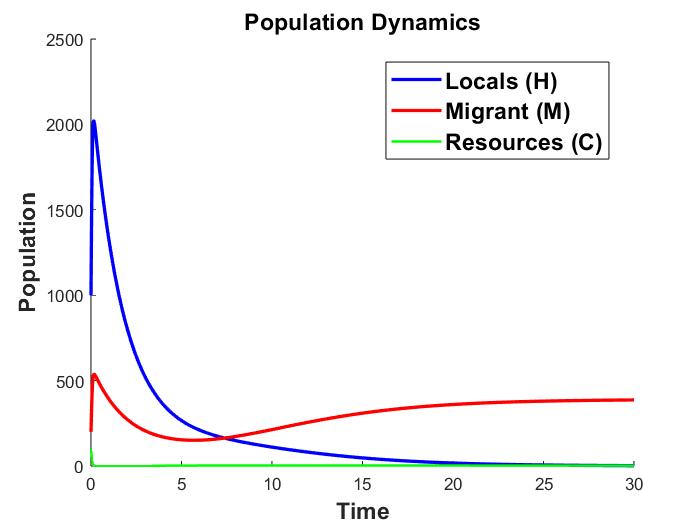
\includegraphics[width=1\linewidth]{5.1.png}
    \caption{Динамика c $H_0 = 1000, \ M_0 = 100, \ \frac{d_H}{f_H} = 4, \frac{d_H}{f_H} = 2.5, \ g = 10, \ r = 0.1$.}
\end{figure}

\subsubsection{Модель c постоянным потоком}

Рассмотрим случай с постоянным потоком мигрантов. При $\mu > 0$ стационарное состояние без мигрантов невозможно ($\frac{dM}{dt}$ всегда больше 0). Найдём условия существования стационара со всеми положительными компонентами.

Из условия $\dfrac{dH}{dt}=0$ при $H > 0$ получаем:

\begin{equation}
    C = \frac{d_H}{f_H}.
\end{equation}

Из условия $\dfrac{dM}{dt}=0$ находим:

\begin{equation}
    M = \frac{\mu}{d_M - f_M C} = \frac{\mu}{d_M - f_M \frac{d_H}{f_H}}.
\end{equation}

Для существования положительного $M$ необходимо:

\begin{equation}
    d_M - f_M \frac{d_H}{f_H} > 0 \quad \Longleftrightarrow \quad \frac{d_M}{f_M} > \frac{d_H}{f_H}.
\end{equation}

Из условия $\dfrac{dC}{dt}=0$ получаем:

\begin{equation}
    H = \frac{1}{e_H}\left( \frac{g}{C} - r - e_M M \right) = \frac{1}{e_H}\left( \frac{g f_H}{d_H} - r - e_M M \right).
\end{equation}

Условие $H > 0$ накладывает ограничение на поток мигрантов:

\begin{equation}
    \mu < \frac{1}{e_M} \left( \frac{g f_H}{d_H} - r \right) \left( d_M - \frac{f_M d_H}{f_H} \right).
\end{equation}

Таким образом, сосуществование при $\mu > 0$ возможно только при выполнении условий:

\begin{enumerate}
    \item Местная популяция более эффективна: $\frac{d_H}{f_H} < \frac{d_M}{f_M}$
    \item Поток мигрантов не превышает критического значения
\end{enumerate}

Таким образом, стационарное состояние одиночной популяции может потерять устойчивость при добавлении мигрантов, если параметры мигрирующей популяции допускают её рост при данном уровне ресурса.

\newpage

\section*{Заключение}
\addcontentsline{toc}{section}{Заключение}

Были рассмотрены ключевые модели популяционной динамики: экспоненциального роста, логистического роста и улучшенные варианты последней.

Основным практическим результатом работы стала программная реализация логистической модели с переменной ёмкостью среды для описания динамики численности аграрного общества в среде MATLAB. 

Полученные знания и результаты являются ценным опытом для дальнейшей деятельности в области математического моделирования в  биологии, экологии и демографии.

\newpage    

\section*{Список литературы}
\addcontentsline{toc}{section}{Список литературы}

\begin{enumerate}
    \item Мюррей Дж. Математическая биология. Том І. Введение. — М.-Ижевск: НИЦ «Регулярная и хаотическая динамика», Институт компьютерных исследований, 2009. — 776 с.

    \item Ризниченко Г. Ю. Лекции по математическим моделям в биологии. — 2-е изд. испр. и доп. — М.– Ижевск: Институт компьютерных исследований, НИЦ «Регулярная и хаотическая динамика», 2010. — 560 с. 

    \item Долбик-Воробей, Татьяна Александровна. Статистика населения и демография + eПриложение: тесты : учебник / Т.А. Долбик-Воробей, О.Д. Воробьева. — Москва : КНОРУС, 2018. — 314 с. — (Магистратура).

    \item Нефедов С. А. Концепция демографических циклов. -Екатеринбург: Издательство УГГУ, 2007. – 141 с.

    \item Евдокимов Е.В. Динамика популяций в задачах и решениях: Учеб. пособие Томск:Томский государственный университет. 2001. 73 с
\end{enumerate}

\newpage

\section*{Приложения}
\addcontentsline{toc}{section}{Приложения}

\appendix

\renewcommand{\appendixname}{Приложение}
\renewcommand{\thesection}{\arabic{section}.}

\subsection{Имплементация аграрной модели в MATLAB}

\begin{lstlisting}[language=matlab, caption={Модель с производством ресурсов.}]
% Parameters
r = 0.015; % Maximum natural population growth rate
a = 650; % Constant related to sowing area
d = 500; % Parameter related to carrying capacity
N0 = 100; % Initial population size
K0 = 50; % Initial grain reserves
Y0 = [N0; K0];
tspan = [0 500];

% Solving the system of differential equations
[t, Y] = ode45(@(t, Y) population_model(t, Y, r, a, d), tspan, Y0);
N = Y(:, 1); % Population over time
K = Y(:, 2); % Grain reserves over time

% Plotting the results
figure;
semilogy(t, N, 'b-', t, K, 'r-');
xlabel('Time');
ylabel('Population (N) and grain reserves (K)');
legend('Population (N)', 'Grain reserves (K)');
title('Logistic model of population size in an agrarian society');
grid on;

% Function describing the system of differential equations
function dY = population_model(t, Y, r, a, d)
    % Extract state variables
    N = Y(1); K = Y(2); % Population and grain reserves
    % Define the system of equations and return derivatives
    dNdt = r * N * (1 - N/K);
    dKdt = (a * N) / (N + d) - N;
    dY = [dNdt; dKdt];
end
\end{lstlisting}

\newpage

\subsection{Простая модель <<ресурс-потребитель>>}

Составим элементарную систему:

\begin{equation}
    \begin{cases}
        \begin{aligned}
        \frac{dx}{dt} &= \lambda - d_x \cdot x \quad &\text{(22) -- динамика ресурса} \\
        \frac{dy}{dt} &= a \cdot x - d_y \cdot y \quad &\text{(23) -- динамика потребителя}
        \end{aligned}
    \end{cases}
\end{equation}

\begin{figure}[H]
\centering
\includesvg[width=0.75\textwidth]{simplest.drawio.svg}
\caption{Схема базовой модели.}
\end{figure}

Cмысл параметров:

\begin{itemize}
    \item $x$ - количество ресурса
    \item $y$ - потребление ресурса  
    \item $\lambda$ - постоянный приток ресурса
    \item $d_x$ - скорость естественной убыли ресурса
    \item $a$ - эффективность потребления
    \item $d_y$ - снижение потребления
\end{itemize}

Описываемое моделью явление: потребление ресурса с определённой интенсивностью. В этом варианте нет обратной связи в виде изменения численности ресурса вследствие увеличения или снижения численности потребителя: влияние потребителя на ресурс пренебрежимо мало либо отсутствует. По этой причине нет смысла рассматривать её как экологическую. Тем не менее, с помощью такой модели можно поверхностно рассмотреть, например, получение электроэнергии при использовании солнечных панелей или ветряных турбин, тогда:

\begin{itemize}
    \item $x$ - энергия ветра или интенсивность света
    \item $y$ - скорость преобразования $x$ в полезную энергию
    \item $\lambda$ - средняя инсоляция или скорость ветра
    \item $d_x$ - естественные потери энергии (облачность, изменение направления ветра)
    \item $a$ - эффективность преобразования
    \item $d_y$ - износ механизма преобразования энергии
\end{itemize}

\newpage

\subsection{Анализ устойчивости модели «ресурс-потребитель»}

Вводим возмущения вокруг стационарной точки ($C_0$, $H_0$) отличной от (0,0). Нужно сказать, что последняя существует только при $g = 0$; фазовым портретом является асимптотически устойчивый узел, ведь два собственных значения $-r, -d_H < 0$:

\begin{equation}
    \begin{cases}
        \begin{aligned}
            C(t) &= C_0 + C'(t) \\
            H(t) &= H_0 + H'(t)
        \end{aligned}
    \end{cases}
\end{equation}

где $C'(t), H'(t)$ -- малые отклонения.

Проведём подробную линеаризацию системы. Запишем исходные уравнения в общем виде:

\begin{equation}
    \begin{cases}
        \begin{aligned}
            F(C,H) &= g - r C - e C H \quad &\text{(24)} \\
            G(C,H) &= f C H - d_H H \quad &\text{(25)}
        \end{aligned}
    \end{cases}
\end{equation}

Разлагаем в ряд Тейлора вокруг точки $(C_0, H_0)$, сохраняя только линейные члены:

\begin{equation}
    \begin{cases}
        \begin{aligned}
    \frac{dC}{dt} &= F(C_0 + C', H_0 + H') \approx F(C_0, H_0) + \frac{\partial F}{\partial C}C' + \frac{\partial F}{\partial H}H' \\
    \frac{dH}{dt} &= G(C_0 + C', H_0 + H') \approx G(C_0, H_0) + \frac{\partial G}{\partial C}C' + \frac{\partial G}{\partial H}H'
        \end{aligned}
    \end{cases}
\end{equation}

Но $F(C_0, H_0) = 0$ и $G(C_0, H_0) = 0$ (стационарная точка), поэтому:

\begin{equation}
    \begin{cases}
        \begin{aligned}
    \frac{dC'}{dt} &= \frac{\partial F}{\partial C}C' + \frac{\partial F}{\partial H}H' \\
    \frac{dH'}{dt} &= \frac{\partial G}{\partial C}C' + \frac{\partial G}{\partial H}H'
        \end{aligned}
    \end{cases}
\end{equation}

Вычисляем частные производные:

\begin{equation}
    \begin{cases}
        \begin{aligned}
    \frac{\partial F}{\partial C} &= -r - e H_0 \\
    \frac{\partial F}{\partial H} &= -e C_0 \\
    \frac{\partial G}{\partial C} &= f H_0 \\
    \frac{\partial G}{\partial H} &= f C_0 - d_H
        \end{aligned}
    \end{cases}
\end{equation}

Для нетривиальной стационарной точки $(C_0, H_0)$, где 

\[
C_0 = \frac{d_H}{f}, \qquad 
H_0 = \frac{f g - r d_H}{e d_H} = \frac{r}{e}(R_0 - 1),
\]

(условие $H_0 > 0$ эквивалентно $R_0 > 1$),подставим ее координаты в частные производные:

\begin{equation}
    \begin{cases}
        \begin{aligned}
    j_{11} &= -r - e H_0 \\
    j_{12} &= -e C_0 \\
    j_{21} &= f H_0 \\
    j_{22} &= f C_0 - d_H = 0 
        \end{aligned}
    \end{cases}
\end{equation}

Таким образом, линеаризованная система имеет вид:

\begin{equation}
    \begin{cases}
        \begin{aligned}
    \frac{dC'}{dt} &= (-r - e H_0) C' + (-e C_0) H' \\
    \frac{dH'}{dt} &= (f H_0) C' + (0) H'
        \end{aligned}
    \end{cases}
\end{equation}

В матричной форме:

\[
\begin{bmatrix} \frac{dC'}{dt} \\ \frac{dH'}{dt} \end{bmatrix} = 
\begin{bmatrix} 
    -r - e H_0 & -e C_0 \\ 
    f H_0 & 0 
\end{bmatrix}
\begin{bmatrix} C' \\ H' \end{bmatrix}
\]

Характеристическое уравнение: $\det(J - sI) = 0$.

\begin{align*}
    \det \begin{bmatrix} 
        -r - e H_0 - s & -e C_0 \\ 
        f H_0 & -s 
    \end{bmatrix} &= 0 \\
    (-r - e H_0 - s)(-s) - (-e C_0)(f H_0) &= 0 \\
    s^2 + (r + e H_0)s + e f C_0 H_0 &= 0 \quad \text{(26)}
\end{align*}

Для стационарной точки $(C_0, H_0) = (g/r, 0)$, подставим её координаты:

\begin{equation}
    \begin{cases}
        \begin{aligned}
    j_{11} &= -r \\
    j_{12} &= -e g/r \\
    j_{21} &= 0 \\
    j_{22} &= f g/r - d_H = d_H(R_0 - 1)
        \end{aligned}
    \end{cases}
\end{equation}

Матрица Якоби:

\[
J(g/r, 0) = 
\begin{bmatrix} 
    -r & -e g/r \\ 
    0 & d_H(R_0 - 1)
\end{bmatrix}
\]

Характеристическое уравнение:

\[
(-r - s)\,(d_H(R_0 - 1) - s)=0.
\]

Собственные значения:

\[
s_1 = -r < 0, \qquad s_2 = d_H(R_0 - 1).
\]

\begin{itemize}
    \item При $R_0 < 1$: $s_2 < 0$ — точка $(g/r,0)$ устойчива.
    \item При $R_0 > 1$: $s_2 > 0$ — точка $(g/r,0)$ является седлом.
    \item При $R_0 = 1$: $s_2 = 0$ — линеаризация не даёт ответа.
\end{itemize}

\newpage

\subsection{Логистическая модель двух популяций с общей ёмкостью среды}

Рассмотрим пример, для которого использование простой логистической модели не вполне корректно: две популяции, конкурирующие за один и тот же ограниченный ресурс. В этом случае логистический рост для каждой из них модифицируется с учётом суммарной численности, потребляющей ресурсы. Система уравнений принимает вид:

\begin{align}
    \frac{dn_1}{dt} &= r_1 \cdot n_1 \cdot \left(1 - \frac{n_1 + n_2}{K}\right) \label{eq:two_pop_1} \\
    \frac{dn_2}{dt} &= r_2 \cdot n_2 \cdot \left(1 - \frac{n_1 + n_2}{K}\right) \label{eq:two_pop_2}
\end{align}

где \(K\) — ёмкость среды. Популяция с более высокой скоростью роста $r$ будет получать преимущество. Для анализа удобно ввести суммарную численность \(N = n_1 + n_2\) и долю второй популяции \(f = n_2 / N\). После преобразований получаем уравнение для доли \(f\):

Обе популяции конкурируют за общий «объем жизненного пространства». Вводим более удобные переменные:

\begin{align}
    N &= n_1 + n_2 &\text{-- общая численность} \label{eq:N_def} \\
    f &= \frac{n_2}{N} &\text{-- доля второй популяции} \label{eq:f_def}
\end{align}

Тогда:

\begin{align}
    n_1 &= (1 - f) \cdot N \label{eq:n1_fN} \\
    n_2 &= f \cdot N \label{eq:n2_fN}
\end{align}

Дифференцируем $f = \frac{n_2}{N}$:

\begin{align}
    \frac{df}{dt} &= \frac{d}{dt}\left(\frac{n_2}{N}\right) = \frac{1}{N} \cdot \frac{dn_2}{dt} - \frac{n_2}{N^2} \cdot \frac{dN}{dt} \label{eq:df_dt_init}
\end{align}

Но $\frac{dN}{dt} = \frac{dn_1}{dt} + \frac{dn_2}{dt}$, поэтому:

\begin{align}
    \frac{df}{dt} &= \frac{N \cdot \frac{dn_2}{dt} - n_2\left(\frac{dn_1}{dt} + \frac{dn_2}{dt}\right)}{N^2} \nonumber = \frac{n_1 \cdot \frac{dn_2}{dt} - n_2 \cdot \frac{dn_1}{dt}}{N^2} \label{eq:df_dt_s}
\end{align}

Подстановка исходных уравнений из \eqref{eq:two_pop_1} - \eqref{eq:two_pop_2}:

\begin{align}
    \frac{dn_1}{dt} &= r_1 \cdot n_1 \cdot \left(1 - \frac{N}{K}\right) \label{eq:dn1_dt_N} \\
    \frac{dn_2}{dt} &= r_2 \cdot n_2 \cdot \left(1 - \frac{N}{K}\right) \label{eq:dn2_dt_N}
\end{align}

Подставляем в \eqref{eq:df_dt_s}:

\begin{align}
    \frac{df}{dt} &= \frac{n_1 \cdot r_2 \cdot n_2 \cdot \left(1 - \frac{N}{K}\right) - n_2 \cdot r_1 \cdot n_1 \cdot \left(1 - \frac{N}{K}\right)}{N^2} \nonumber \\
    &= \frac{n_1 \cdot n_2}{N^2} \cdot \left(1 - \frac{N}{K}\right) \cdot (r_2 - r_1) \label{eq:df_dt_intermediate}
\end{align}

Учитывая что $\frac{n_1 \cdot n_2}{N^2} = \frac{(1-f)N \cdot fN}{N^2} = f(1-f)$, получаем:

\begin{align}
    \frac{df}{dt} &= f(1-f) \cdot \left(1 - \frac{N}{K}\right) \cdot \Delta r \label{eq:df_dt_final}
\end{align}

где $\Delta r = r_2 - r_1$

Уравнение для общей численности:

\begin{align}
    \frac{dN}{dt} &= \frac{dn_1}{dt} + \frac{dn_2}{dt} \nonumber = r_1 \cdot n_1 \cdot \left(1 - \frac{N}{K}\right) + r_2 \cdot n_2 \cdot \left(1 - \frac{N}{K}\right) \nonumber \\
    &= \left(1 - \frac{N}{K}\right) \cdot [r_1 \cdot (1-f)N + r_2 \cdot fN] \nonumber
\end{align}

\begin{align}
    \frac{dN}{dt} &= N \cdot \left(1 - \frac{N}{K}\right) \cdot [r_1(1-f) + r_2 f] \label{eq:dN_dt_final}
\end{align}

Система \eqref{eq:df_dt_final}-\eqref{eq:dN_dt_final} представляет серьезную математическую проблему: уравнение \eqref{eq:df_dt_final} для $f$ содержит $N$, а уравнение \eqref{eq:dN_dt_final} для $N$ содержит $f$. Это связанная система, не допускающая разделения переменных в обычном смысле. Динамика долей популяций и общей численности взаимно влияют друг на друга. Чтобы множитель $\left(1 - \frac{N}{K}\right)$ не мешал интегрированию, нужно ввести новую временную переменную. Зададим новое время $T$:

\begin{align}
    dT = \left(1 - \frac{N(t)}{K}\right) \cdot dt \label{eq:dT_def}
\end{align}

Это «эффективное конкурентное время». $T$ течет пропорционально «свободному пространству» в среде:
\begin{itemize}
    \item Когда $N \ll K$ (много свободного места), $dT \approx dt$ -- время течет нормально
    \item Когда $N \to K$ (емкость насыщена), $dT \to 0$ -- время «замедляется»
\end{itemize}

$T$ измеряет «накопленную конкурентную нагрузку» на среду. Важно понимать, что преобразование корректно пока $N < K$ (положительное время).

Используем правило производной сложной функции:

\begin{align}
    \frac{df}{dT} &= \frac{df/dt}{dT/dt} = \frac{f(1-f) \cdot \left(1 - \frac{N}{K}\right) \cdot \Delta r}{\left(1 - \frac{N}{K}\right)} \nonumber = f(1-f) \cdot \Delta r \label{eq:df_dT_simple}
\end{align}

Результат: в новых переменных уравнение для доли существенно упростилось! Уравнение \eqref{eq:df_dT_simple} -- это логистическое уравнение:

\begin{align}
    \frac{df}{dT} = \Delta r \cdot f(1-f) \label{eq:logistic_T}
\end{align}

Разделяем переменные:

\begin{align}
    \int \frac{df}{f(1-f)} = \int \Delta r  dT \label{eq:separation}
\end{align}

Раскладываем на простые дроби (метод неопределенных коэффициентов):

\begin{align}
    \frac{1}{f(1-f)} = \frac{A}{f} + \frac{B}{1-f} \label{eq:partial_fractions}
\end{align}

Находим $A$ и $B$:

\begin{align}
    A(1-f) + Bf &= 1 \nonumber \\
    A + (B-A)f &= 1 \quad \Rightarrow \quad A = 1, B = 1 \label{eq:coeffs_AB}
\end{align}

Таким образом:

\begin{align}
    \frac{1}{f(1-f)} = \frac{1}{f} + \frac{1}{1-f} \label{eq:partial_result}
\end{align}

Вычисление интегралов:

\begin{align}
    \int \frac{df}{f} + \int \frac{df}{1-f} &= \Delta r \cdot T + C \nonumber \\
    \ln|f| - \ln|1-f| &= \Delta r \cdot T + C \nonumber \\
    \ln\left|\frac{f}{1-f}\right| &= \Delta r \cdot T + C \label{eq:log_ratio}
\end{align}

Потенцирование:

\begin{align}
    \ln\left|\frac{f}{1-f}\right| &= \Delta r \cdot T + C \nonumber \\
    \exp\left(\ln\left|\frac{f}{1-f}\right|\right) &= \exp(\Delta r \cdot T + C) \nonumber \\
    \left|\frac{f}{1-f}\right| &= e^{\Delta r \cdot T} \cdot e^C \label{eq:exp_ratio}
\end{align}

Поскольку $f$ и $1-f$ > 0 (доли популяций), модули можно опустить:

\begin{align}
    \frac{f}{1-f} &= e^C \cdot e^{\Delta r \cdot T} \label{eq:ratio_no_abs}
\end{align}

Обозначим $C' = e^C$:

\begin{align}
    \frac{f}{1-f} &= C' \cdot e^{\Delta r \cdot T} \label{eq:ratio_Cprime}
\end{align}

При $T = 0$ ($t = 0$) имеем $f = f_0$:

\begin{align}
    \frac{f_0}{1-f_0} &= C' \cdot e^0 = C' \nonumber \\
    C' &= \frac{f_0}{1-f_0} \label{eq:Cprime_value}
\end{align}

Подставляем в \eqref{eq:ratio_Cprime}:

\begin{align}
    \frac{f}{1-f} &= \frac{f_0}{1-f_0} \cdot e^{\Delta r \cdot T} \label{eq:ratio_with_initial}
\end{align}

Выражаем $f$:

\begin{align}
    f &= (1-f) \cdot \frac{f_0}{1-f_0} \cdot e^{\Delta r \cdot T} \nonumber \\
    f &= \frac{f_0}{1-f_0} \cdot e^{\Delta r \cdot T} - f \cdot \frac{f_0}{1-f_0} \cdot e^{\Delta r \cdot T} \nonumber \\
    f &= \frac{\frac{f_0}{1-f_0} \cdot e^{\Delta r \cdot T}}{1 + \frac{f_0}{1-f_0} \cdot e^{\Delta r \cdot T}} \nonumber \\
    f(T) &= \frac{1}{1 + \frac{1-f_0}{f_0} \cdot e^{-\Delta r \cdot T}} \label{eq:f_T_form1}
\end{align}

Или в более симметричной форме:

\begin{align}
    f(T) &= \frac{f_0}{f_0 + (1-f_0) \cdot e^{-\Delta r \cdot T}} \label{eq:f_T_form2}
\end{align}

Проанализируем полученный результат:

\begin{itemize}
    \item При $\Delta r > 0$ ($r_2 > r_1$): вторая популяция вытесняет первую, $f \to 1$
    \item При $\Delta r < 0$ ($r_2 < r_1$): первая популяция вытесняет вторую, $f \to 0$  
    \item При $\Delta r = 0$: доли остаются постоянными
\end{itemize}

Из определения \eqref{eq:dT_def}: $T = \int_0^t \left[1 - \frac{N(\tau)}{K}\right] d\tau$

Таким образом, «эффективное время» $T$ течет медленнее реального времени $t$ когда популяция близка к емкости среды ($N \approx K$).

Система имеет три типа стационарных точек:

\begin{enumerate}
\item Тривиальное равновесие: \(E_0 = (0, 0)\) — обе популяции вымерли. 
\begin{itemize}
\item Матрица Якоби: \(J = \begin{bmatrix} r_1 & 0 \\ 0 & r_2 \end{bmatrix}\)
\item Собственные значения: \(\lambda_1 = r_1 > 0\), \(\lambda_2 = r_2 > 0\)
\item Неустойчивый узел при \(r_1, r_2 > 0\)
\end{itemize}

\item Одна популяция вымерла: \(E_1 = (K, 0)\) и \(E_2 = (0, K)\)
\begin{itemize}
\item Для \(E_1 = (K, 0)\): \(J = \begin{bmatrix} -r_1 & -r_1 \\ 0 & r_2(1-\frac{K}{K}) \end{bmatrix} = \begin{bmatrix} -r_1 & -r_1 \\ 0 & 0 \end{bmatrix}\)
\item Собственные значения: \(\lambda_1 = -r_1 < 0\), \(\lambda_2 = 0\)
\item Точки безразличного равновесия.
\item Аналогично для \(E_2 = (0, K)\)
\end{itemize}

\item Линия сосуществования: \(n_1 + n_2 = K\) при любом соотношении $n_1$ и $n_2$
\begin{itemize}
\item На всей этой линии выполняется условие $N = K$, что означает полное заполнение ёмкости среды
\item При этом $\frac{dn_1}{dt} = \frac{dn_2}{dt} = 0$ для любых положительных $n_1, n_2$, удовлетворяющих $n_1 + n_2 = K$
\item Матрица Якоби на линии: \(J = \begin{bmatrix} -r_1\frac{n_1}{K} & -r_1\frac{n_1}{K} \\ -r_2\frac{n_2}{K} & -r_2\frac{n_2}{K} \end{bmatrix}\)
\item Собственные значения: \(\lambda_1 = 0\), \(\lambda_2 = -(r_1\frac{n_1}{K} + r_2\frac{n_2}{K}) < 0\)
\item Это линия безразличного равновесия.
\end{itemize}
\end{enumerate}

\begin{figure}[h]
    \centering
    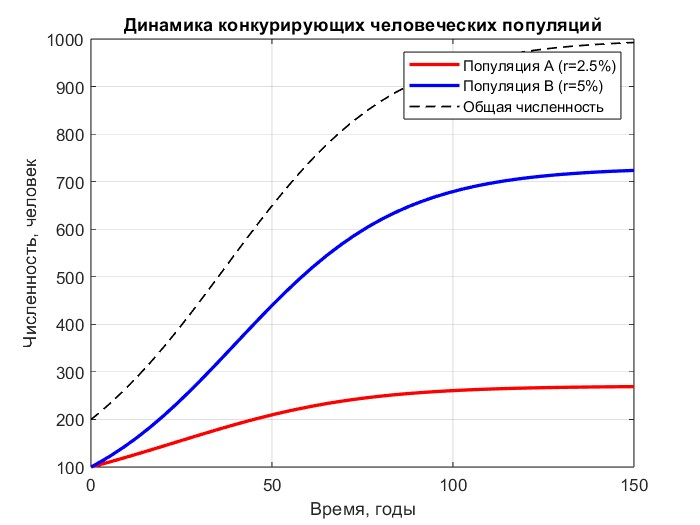
\includegraphics[width=0.85\linewidth]{2_pops.jpg}
    \caption{При \(r_1=0.025, r_2=0.05, K=1000\) популяции сосуществуют и достигают <<потолка>> через $\approx 150$ лет.}
\end{figure}

Хотя модель с общей ёмкостью среды корректно описывает суммарный рост двух популяций, она принципиально не отражает механизма конкуренции между ними. В ней обе популяции воздействуют на ресурс одинаковым способом: каждая особь любого вида уменьшает <<свободное место>> в среде так же, как особь другого вида. Поэтому конкурентное взаимодействие здесь симметрично и не зависит от того, как именно виды используют ресурс. 

В результате единственный источник различий — параметры $r_1$ и $r_2$, и модель не содержит механизма, который мог бы приводить к вытеснению одного вида другим в смысле принципа Гаузе.

\newpage

\subsection{Логистическая модель с разделёнными экологическими нишами}

Две популяции используют пересекающиеся, но не идентичные ресурсы. Это приводит к системе с раздельными ёмкостями:

\begin{equation}
\begin{cases}
\dfrac{dn_1}{dt} = r_1 n_1 \left( 1 - \dfrac{n_1 + \alpha_{12} n_2}{K_1} \right) \\
\dfrac{dn_2}{dt} = r_2 n_2 \left( 1 - \dfrac{n_2 + \alpha_{21} n_1}{K_2} \right)
\end{cases}
\label{eq:separate_niches}
\end{equation}

Параметр \(\alpha_{12}\) (или \(\alpha_{21}\)) — коэффициент конкуренции; он показывает, насколько одна особь вида 2 эквивалентна по своему влиянию на ресурсы вида 1 особям вида 1. Например, если \(\alpha_{12} = 0.5\), то каждая особь вида 2 создаёт такую же нагрузку на ресурсы вида 1, как 0.5 особи вида 1.

Найдём стационарные точки. В стационарном состоянии (\(dn_1/dt = 0\), \(dn_2/dt = 0\)) при ненулевых численностях получаем:

\begin{equation}
\begin{cases}
n_1 + \alpha_{12} n_2 = K_1 \label{eq:stationary_a} \\
\alpha_{21} n_1 + n_2 = K_2 \label{eq:stationary_b}
\end{cases}
\end{equation}

В равновесии общая <<нагрузка>> на среду для каждой популяции равна её ёмкости.

Решаем систему. Из уравнения \eqref{eq:stationary_a} выражаем \(n_1\):

\[
n_1 = K_1 - \alpha_{12} n_2
\]

Подставляем в \eqref{eq:stationary_b}:

\[
\alpha_{21}(K_1 - \alpha_{12} n_2) + n_2 = K_2
\]

Раскрываем скобки и группируем:

\begin{align}
    \alpha_{21} K_1 - \alpha_{21} \alpha_{12} n_2 + n_2 &= K_2 \nonumber \\
    n_2 (1 - \alpha_{12} \alpha_{21}) &= K_2 - \alpha_{21} K_1 \nonumber
\end{align}

Получаем стационарную численность второй популяции:

\begin{equation}
n_2^* = \dfrac{K_2 - \alpha_{21} K_1}{1 - \alpha_{12} \alpha_{21}} \label{eq:n2_star}
\end{equation}

Аналогично, подставляя в уравнение для \(n_1\):

\begin{equation}
n_1^* = \dfrac{K_1 - \alpha_{12} K_2}{1 - \alpha_{12} \alpha_{21}} \label{eq:n1_star}
\end{equation}

Для существования равновесия с положительными численностями необходимо:

\[
n_1^* > 0 \quad \text{и} \quad n_2^* > 0
\]

Это выполняется при:

\begin{equation}
\begin{cases}
K_1 > \alpha_{12} K_2 \\
K_2 > \alpha_{21} K_1 \\
1 - \alpha_{12} \alpha_{21} > 0
\end{cases}
\label{eq:coexistence_conditions}
\end{equation}

То есть, каждая популяция должна иметь достаточную собственную ёмкость, чтобы <<поделиться>> с конкурентом.

Проведём анализ устойчивости. Имеем систему второго порядка. Матрица Якоби системы имеет вид:

\begin{equation}
J = \begin{bmatrix}
-\dfrac{r_1 n_1^*}{K_1} & -\dfrac{r_1 \alpha_{12} n_1^*}{K_1} \\[0.5em]
-\dfrac{r_2 \alpha_{21} n_2^*}{K_2} & -\dfrac{r_2 n_2^*}{K_2}
\end{bmatrix}
\label{eq:jacobian_matrix}
\end{equation}

Характеристическое уравнение для собственных значений \(\lambda\):

\[
\det(J - \lambda I) = 0
\]

Раскрывая определитель, получаем:

\begin{equation}
\lambda^2 - \text{tr}(J)\lambda + \det(J) = 0
\label{eq:characteristic_eq_full}
\end{equation}

где:
\[
\text{tr}(J) = -\left(\dfrac{r_1 n_1^*}{K_1} + \dfrac{r_2 n_2^*}{K_2}\right), \quad
\det(J) = \dfrac{r_1 r_2 n_1^* n_2^*}{K_1 K_2}(1 - \alpha_{12} \alpha_{21})
\label{eq:trace_det}
\]

Корни уравнения \eqref{eq:characteristic_eq_full} равны:
\[
\lambda_{1,2} = \frac{\text{tr}(J) \pm \sqrt{\text{tr}(J)^2 - 4\det(J)}}{2}
\]

Проанализируем все возможные случаи:

\begin{enumerate}
\item Действительные различные корни (\(\text{tr}(J)^2 > 4\det(J)\)): оба корня < 0, если \(\text{tr}(J) < 0\) и \(\det(J) > 0\)

\item Комплексные корни (\(\text{tr}(J)^2 < 4\det(J)\)): действительная часть корней: \(\text{Re}(\lambda) = \frac{\text{tr}(J)}{2}\) < 0 при \(\text{tr}(J) < 0\).

\item Кратные корни (\(\text{tr}(J)^2 = 4\det(J)\)): \(\lambda = \frac{\text{tr}(J)}{2}\) < 0 при \(\text{tr}(J) < 0\)
\end{enumerate}

Таким образом, критерий устойчивости: 
\[
\text{tr}(J) < 0 \quad \text{и} \quad \det(J) > 0
\]

В нашей системе условие \(\text{tr}(J) < 0\) выполняется всегда при положительных параметрах, а условие \(\det(J) > 0\) требует:

\begin{equation}
1 - \alpha_{12} \alpha_{21} > 0 \quad \Rightarrow \quad \alpha_{12} \alpha_{21} < 1
\label{eq:stability_condition}
\end{equation}

Это означает, что оба собственных значения имеют отрицательные действительные части, что гарантирует устойчивость стационарной точки. Условие \eqref{eq:stability_condition} означает, что устойчивое сосуществование возможно, когда межпопуляционная конкуренция слабее внутрипопуляционной.

Несмотря на кажущуюся применимость, модель с разделёнными ёмкостями, которая является естественным расширением логистической динамики на случай двух конкурирующих видов, довольно ограниченна. Коэффициенты $\alpha_{12}, \alpha_{21}$ превращают влияние одного вида на другой в простое «добавление нагрузки» к его собственной численности. 

\begin{figure}[H]
    \centering
    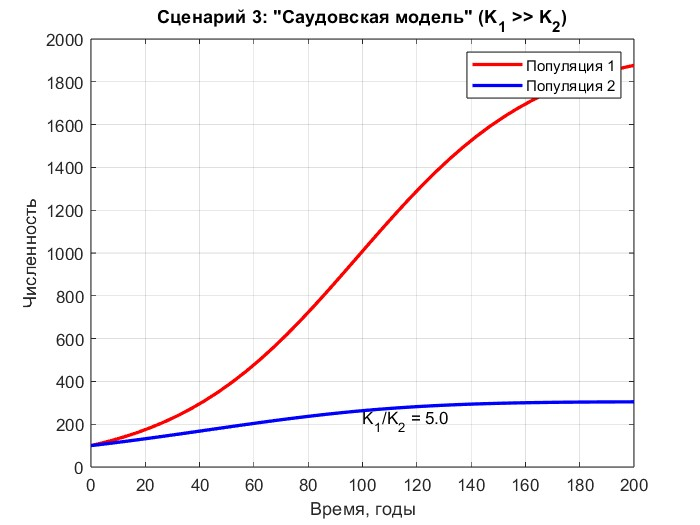
\includegraphics[width=1\linewidth]{saudi.jpg}
    \caption{При $r_1=0.03, r_2=0.02, K_1=2000, K_2 = 400$, и $\alpha_{12} \alpha_{21} < 0.1 \cdot 0.05 << 1$ популяции сосуществуют, не доходя до <<потолка>> своих ниш}
\end{figure}

Такое представление предполагает, что оба вида воздействуют на один и тот же набор ресурсов линейно и одинаковым способом, различаясь только масштабом этого воздействия. В действительности же конкуренция возникает из взаимодействия популяций с конкретными ресурсами, и сила влияния одного вида на другой определяется структурой потребления ресурсов, а не абстрактной нагрузкой на ёмкость. Поэтому данная система является частным случаем более общей ресурсной модели, в которой взаимодействия задаются матрицей коэффициентов потребления.

\end{document}